
\chapwithtoc{Introduction}
\label{sec:Introduction}

An \lsystem (also called a Lindenmayer system) is a mathematical formalism that was developed by Aristid Lindenmayer in 1968 for modeling plant growth~\cite{Lin68}.
An example of a plant modeled by an \lsystem is shown in \autoref{fig:introLilac}.
In its simplest form an \lsystem is a variant of a regular or \mbox{context-free} grammar.
By rewriting (deriving) an initial string of symbols (also called an axiom) with some rewrite rules from a grammar, an \lsystem produces a new string of symbols which can be interpreted in many different ways.
In the first \lsystems by used Lindenmayer there symbols were to be interpreted as cells of algae.
Later, different approach was adopted by Przemyslaw Prusinkiewicz who interpreted the \lsystem symbols using \mbox{Logo-like} turtle drawing system%
	\footnote{Logo a is computer programming language developed for use in the education of programming for children.
	Logo controls a cybernetic turtle which does the drawing on a 2D canvas.}~\cite{Pru85}.
With this method he obtained more plant-like structures and fractals~\cite{CD93}.
In \autoref{fig:introHTree} you can see a H-tree fractal created by an \lsystem.

\begin{figure}[h!]
	\subfloat[Model of lilac panicle]{
		\includegraphics[width=0.49\linewidth]{lilac}
		\label{fig:introLilac}
	} \hfill
	\subfloat[H-tree fractal]{
		
\includegraphics[width=0.49\linewidth]{HTree}
		\label{fig:introHTree}
	}
	\caption{Examples of models created by an \lsystem}
\end{figure}


Over time \lsystems began to used in many diverse areas.
For example they were used to generate rivers in fractal mountains~\cite{PH93}, streets in virtual cities~\cite{PM01} and to describe the subdivision of curves~\cite{PSSK03}.
\lsystems can be used in fields other than computer graphics: for example, in music generation~\cite{HCJ99, Man06}.
They are still used in plant modeling.
Plant models generated with \lsystems are used in modern video games or films: for example, they were used to generate many plants and trees for the famous film Avatar~\cite{Wor08, Dun10}.~\footnote{\citeauthor{SBM10} presented a reverse method -- the automatic generation of \lsystems from a 2D model~\cite{SBM10}.}

\lsystems have a wide variety of interesting applications but it is not easy to find a place to experiment with them.
Esentially there are two basic types of \lsystem generators: web-based and desktop applications.
Web-based \lsystem generators are easily accessible but they are often too primitive to offer much more than the generation of simple fractals (see \autoref{sec:WebBasedGenerators}).
Some of them do not even work in the most-used browsers.

Desktop applications generally offer more options than web-based ones but most of them are also quite simple and do not offer advanced types of \lsystems.
There are some complex applications that offer pretty good sets of features but these are expensive, not easy to control, and/or they are old and no longer maintained (see \autoref{sec:DesktopGenerators}).
A problem with desktop applications is also their compatibility with a user's operating system, its version, and the libraries installed.

The overall goal of this work is to take the best from both of the two main approaches and an create online, feature-rich, development environment for anybody who wants to experiment with \lsystems.
The development environment will be divided into two parts: a web user interface and an \lsystem processing library.

\begin{wrapfigure}{r}{0.5\textwidth}%
	\vspace{6pt}%
	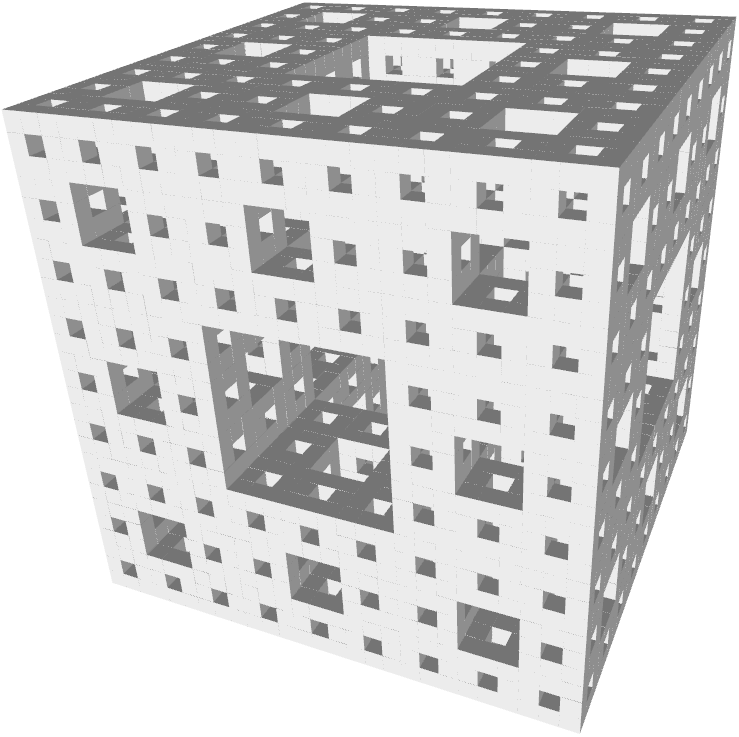
\includegraphics[width=\linewidth]{MengerSponge}
	\caption{Menger sponge created by an \lsystem}
	\label{fig:introMengerSponge}
\end{wrapfigure}

The user interface will be web a site that offers great accessibility.
Anyone from around the world will be able to use it from any device connected to the Internet , such as: computers, laptops, tablets or smart phones.
The interface should be user-friendly to new users and also offer advanced features for experienced users.
The primary output format of the web-based \lsystem processor will be 2D images but it will also be possible to create and display 3D outputs using modern HTML5 WebGL%
	\footnote{WebGL (Web-based Graphics Library) is a cross-platform, royalty-free web standard for a low-level 3D graphics API based on OpenGL ES 2.0, exposed through the HTML5 Canvas element as Document Object Model interfaces.
		WebGL code executes on a computer display card's GPU (graphics processing unit).}
	technology directly in the browser.
In \autoref{fig:introMengerSponge} is a print-screen of a Menger Sponge model displayed by WebGL.
Part of the web site will be a gallery of \lsystems.
Any registered user can add his own \lsystems to the gallery along with a description and then others can rate it.
This will help to create a community of active users and it can also serve as a learning tool for new users.
\nomenclature{HTML5}{hypertext markup language}
\nomenclature{WebGL}{web graphics library}
\nomenclature{API}{application programming interface}
\nomenclature{GPU}{graphics processing unit}

The second part of the application will be the \lsystem processing library.
Although it will be designed to support the demands of a web interface, it will be independent and should be usable in other applications.
During the design of the library, great emphasis will be placed on its ease of extensibility to make it as universal as possible.
It should be possible to extend the library by the users themselves.

A new syntax for input will be designed to improve the user experience especially for new users.
The syntax should be clean, easy to understand and to remember.
%The syntax will cover all needs of library from defining \lsystems to configuring whole processing system.
%This will also ensure that whole input can be written in one file which will simplify source code sharing and saving.
%Parser generator will be used for creating robust and extensible parser.


\section*{Structure of the thesis}

In the first chapter a formal definition of \lsystems is given and principles for their rewriting and interpretation are explained.
Then follows some descriptions of \lsystem types and their properties.
At the end of the first chapter is a list of some related \lsystem generators.

The second chapter is devoted to the design of the solution.
There is described how \lsystem processing library and web user interface works.

Implementation details of the project are discussed in the third chapter.
Sections in this chapters explains individual problems and their solutions.
The text accompanies actual source code snippets and diagrams for better explanation.

The fourth chapter summarizes the results.
Part of this chapter is showcase of images of generated \lsystems.

All the source codes of \lsystems used in this thesis are in a syntax designed as a part of this work.
A reference to this syntax can be found in attachment \ref{chap:syntax}.
It is possible to process all the source code on the web.
More information about the figures in this thesis together with additional information and their source codes is given in attachment \ref{chap:aboutFigures}.































